\documentclass{standalone}

\usepackage{unicode-math} % Euler virtual math fonts.
\usepackage{tikz}

\usetikzlibrary{external}
\usetikzlibrary{arrows.meta} % Advanced arrow tip library.
\usetikzlibrary{calc} % Coordinate calculations.

\definecolor{wwqqcc}{rgb}{0.4, 0, 0.8}
\definecolor{qqzzqq}{rgb}{0, 0.6, 0}
\definecolor{ffwwqq}{rgb}{1, 0.4, 0}

\setmathfont{Euler Math}

\tikzexternalize % activate externalization
\tikzsetnextfilename{mouldUkeita.pdf}

\begin{document}
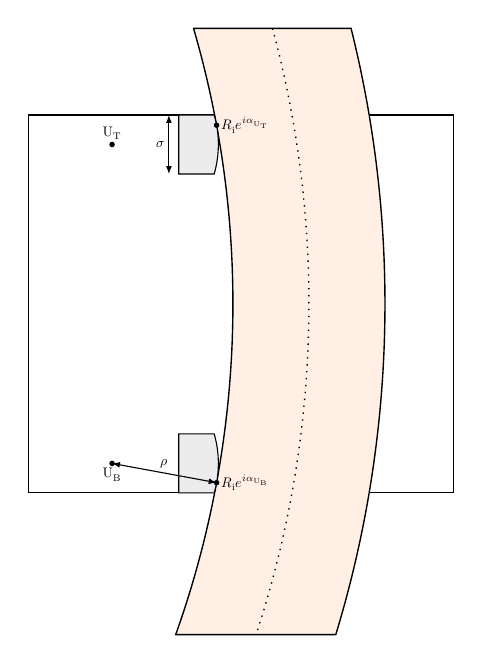
\begin{tikzpicture}[scale=1,
                    every node/.style={scale=0.5},
                    >={Latex[length=1mm, width=0.75mm]},]
% 値の計算
\pgfmathsetmacro{\Ax}{12}                    %A:T_iのx座標
\pgfmathsetmacro{\Ay}{3.5}                   %A:T_iのy座標
\pgfmathsetmacro{\Bx}{2.0+(\Ax)}             %B:T_oのx座標
\pgfmathsetmacro{\Cy}{-4.2}                  %C:B_iのy座標
\pgfmathsetmacro{\TUb}{2.4}                  %TUb:テーブル-モールドの交点y座標
\pgfmathsetmacro{\Ix}{2.7}                   %I:テーブルx方向の長さの半分
\pgfmathsetmacro{\Uw}{0.75}                  %Uw:受板の幅
\pgfmathsetmacro{\Ul}{0.45}                  %Ul:受板の長さ
\pgfmathsetmacro{\Ur}{1.35}                   %Uw:受板の半径
\pgfmathsetmacro{\Ri}{sqrt((\Ax)^2+(\Ay)^2)} %R_iの長さ
\pgfmathsetmacro{\Hx}{0.1+(\Ri)}             %H:テーブルの中心
% 値の計算
\pgfmathsetmacro{\Cx}{sqrt((\Ri)^2-(\Cy)^2)}    %C:B_iのx座標
\pgfmathsetmacro{\Ro}{sqrt((\Bx)^2+(\Ay)^2)}    %R_oの長さ
\pgfmathsetmacro{\Dx}{sqrt((\Ro)^2-(\Cy)^2)}    %D:B_oのx座標
\pgfmathsetmacro{\Rc}{(\Ri+\Ro)/2}              %R_cの長さ
\pgfmathsetmacro{\Ex}{sqrt((\Rc)^2-(\Ay)^2)}    %E:湾曲中心線トップ端のx座標
\pgfmathsetmacro{\Fx}{sqrt((\Rc)^2-(\Cy)^2)}    %F:湾曲中心線ボトム端のx座標
\pgfmathsetmacro{\TUx}{sqrt((\Ri)^2-(\TUb)^2)}  %TUx:テーブル-モールド内側との交点のx座標
\pgfmathsetmacro{\TUxo}{sqrt((\Ro)^2-(\TUb)^2)} %TUxo:テーブル-モールド外側との交点x座標
\pgfmathsetmacro{\Ub}{\Ri*sin(asin((\TUb-\Uw/2)/(\Ri-\Ur)))} %Ub:ボトム側受板-モールド接点のy座標
\pgfmathsetmacro{\Ux}{sqrt((\Ri)^2-(\Ub)^2)}    %Ux:トップ側受板-モールド接点のx座標
\pgfmathsetmacro{\Ucx}{\Ux-sqrt((\Ur)^2-((\Uw)/2-(\TUb-\Ub))^2)} %Uw:受板の半径
\pgfmathsetmacro{\TBUx}{\Ucx+sqrt((\Ur)^2-((\Uw)/2)^2)} %TBUx:テーブルと受板の交点x座標
% 座標の定義
\coordinate (A) at (\Ax, \Ay); %
\coordinate (B) at (\Bx, \Ay);
\coordinate (C) at (\Cx, \Cy);
\coordinate (D) at (\Dx, \Cy);
\coordinate (E) at (\Ex, \Ay);
\coordinate (F) at (\Fx, \Cy);
\coordinate (Ut) at (\Ux, \Ub);
\coordinate (TUt) at (\TUx, \TUb);
\coordinate (Ub) at (\Ux, -\Ub);
\coordinate (TUb) at (\TUx, -\TUb);
\coordinate (TUto) at (\TUxo, \TUb);
\coordinate (TUbo) at (\TUxo, -\TUb);
\coordinate (Tal) at (\Hx-\Ix, \TUb);
\coordinate (Tbl) at (\Hx-\Ix, -\TUb);
\coordinate (Tar) at (\Hx+\Ix, \TUb);
\coordinate (Tbr) at (\Hx+\Ix, -\TUb);
\coordinate (Lt) at (\Hx+\Ix+0.4, \TUb);
\coordinate (Lb) at (\Hx+\Ix+0.4, -\TUb);
\coordinate (Lc) at (\Hx+\Ix+0.4, 0);
\coordinate (Fc) at (\Hx+\Ix+1.0, 0);
\coordinate (TUc) at (\Ucx, \TUb-\Uw/2);
\coordinate (BUc) at (\Ucx, \Uw/2-\TUb);
\coordinate (TTU) at (\TBUx, \TUb);
\coordinate (TTUex) at (\TBUx-\Ul, \TUb);
\coordinate (TUex) at (\TBUx-\Ul, \TUb-\Uw);
\coordinate (TU) at (\TBUx, \TUb-\Uw);
\coordinate (TBU) at (\TBUx, -\TUb);
\coordinate (TBUex) at (\TBUx-\Ul, -\TUb);
\coordinate (BUex) at (\TBUx-\Ul, -\TUb+\Uw);
\coordinate (BU) at (\TBUx, -\TUb+\Uw);
% モールド外形
\draw[line width=0.5pt, fill=ffwwqq, fill opacity=0.1]
  let \p1=(A), \p2=(C), \p3=(B), \p4=(D), \n1={atan2(\y1,\x1)}, \n2={atan2(\y2,\x2)}, \n3={atan2(\y3,\x3)}, \n4={atan2(\y4,\x4)}
    in (A) -- (B) -- (\n3:\Ro) arc (\n3:\n4:\Ro) -- (C) -- (\n2:\Ri) arc (\n2:\n1:\Ri) -- cycle;
% モールド中心線
\draw[dotted, line width=0.5pt] let \p1=(E), \p2=(F), \n1={atan2(\y1,\x1)}, \n2={atan2(\y2,\x2)}
  in (\n1:\Rc) arc (\n1:\n2:\Rc);
% テーブル
\draw (TUt) -- (Tal) -- (Tbl) -- (TUb);
\draw (TUto) -- (Tar) -- (Tbr) -- (TUbo);
% 受板
\draw[fill=gray!15!] let \p1=(TUc), \p2=(TU), \p3=(TTU), \n1={atan2(\y2-\y1,\x2-\x1)}, \n2={atan2(\y3-\y1,\x3-\x1)},
    in (TTU) -- (TTUex) -- (TUex) -- (TU) arc[start angle=\n1, end angle=\n2, radius=\Ur] -- cycle;
\draw[fill=gray!15!] let \p1=(BUc), \p2=(BU), \p3=(TBU), \n1={atan2(\y2-\y1,\x2-\x1)}, \n2={atan2(\y3-\y1,\x3-\x1)},
    in (TBU) -- (TBUex) -- (BUex) -- (BU) arc[start angle=\n1, end angle=\n2, radius=\Ur] -- cycle;
\draw[<->] (BUc) -- (Ub) node[midway, above] {$\rho$};
\draw[<->] ([xshift=-1.25mm]TTUex) -- ([xshift=-1.25mm]TUex) node[midway, left] {$\sigma$};
% 点を描画
\fill (Ut) circle (1pt);
\fill (Ub) circle (1pt);
\fill (TUc) circle (1pt);
\fill (BUc) circle (1pt);
% 点にラベルを付ける
\node at (Ut) [right] {$R_\mathrm ie^{i\alpha_{\mathrm U_\mathrm T}}$};
\node at (Ub) [right] {$R_\mathrm ie^{i\alpha_{\mathrm U_\mathrm B}}$};
\node at (TUc) [above] {U$_\mathrm T$};
\node at (BUc) [below] {U$_\mathrm B$};
\end{tikzpicture}%
\end{document}
